\documentclass[11pt]{article}
\usepackage[a4paper,left=2cm,right=2cm,top=3cm,bottom=3cm,bindingoffset=5mm]{geometry}
\usepackage[german]{babel}
\usepackage[utf8]{inputenc}
\usepackage{graphicx}
\usepackage{caption}
\usepackage{subcaption}
\usepackage{lastpage}
\usepackage{epstopdf}
\graphicspath{outdir=/u/mhemmer/Documents/Theses/BachelorArbeit/}
\usepackage{fancyhdr}
\usepackage{amsmath}
\usepackage{amsthm}
\usepackage{amsbsy}
\usepackage{amssymb}
\usepackage{hyperref}
\usepackage{physics}
\usepackage[doublespacing]{setspace} %fuer Korrektur


\pagestyle{fancy}
\fancyhf{}
\fancyhead[LE,RO]{\thepage}
%\fancyhead[RE,LO]{\leftmark}
\fancyhead[RE,LO]{\rightmark}

\renewcommand{\headrulewidth}{1pt}

\setcounter{section}{0}								%Gliederungsnummerierung faengt bei 0 an.

%opening
%\title{Systematische Studie der Peakextraktion neutraler Pionen in pp-Kollisionen bei $\sqrt{s}=13\text{ TeV}$ mit Hilfe von Templates}
\author{Marvin Hemmer}


\begin{document}

\begin{titlepage}
\begin{center}
\vspace*{1cm}
 
\Huge
\textbf{Systematische Studie der Peakextraktion neutraler Pionen in pp-Kollisionen bei $\sqrt{s}=13\text{ TeV}$ mit Hilfe von Templates}
 
\vspace{3.5cm}
\LARGE
Bachelorarbeit\\
vorgelegt von\\
\textbf{Marvin Hemmer}

\vfill
%\vspace{0.8cm}
 
\Large
am Institut f\"ur Kernphysik\\

\includegraphics[width=0.4\textwidth]{IKF-Logokl}\\
dem Fachbereich Physik\\
der Goethe Universit\"at Frankfurt am Main\\
Januar 2019
 
\end{center}
\end{titlepage}
%\maketitle
\newpage
\tableofcontents
\newpage

\section*{Einleitung}

\section{Theoretische Grundlagen} \label{s1}
\subsection{Standardmodell der Elementarteilchenphysik} \label{s1s1}
Im Standardmodell der Elementarteilchenphysik werden die sogenannten Elementarteilchen in zwei Gruppen, die sogenannten Quarks und die sogenannten Leptonen, unterteilt.
Als Elementarteilchen werden alle Teilchen bezeichnet, die nach heutigem Kenntnisstand nicht weiter teilbar sind.
Beide Gruppen beinhalten nach aktuellem Wissensstand jeweils sechs Teilchen, die sechs Quarks \textit{up} ($u$), \textit{down} ($d$), \textit{charm} ($c$), \textit{strange} ($s$), \textit{top} ($t$) und \textit{bottom} ($b$) und die sechs Leptonen Elektron ($e$), Elektron-Neutrino ($\nu_\text{e}$), Myon ($\mu$), Myon-Neutrino ($\nu_{\mu}$), Tau ($\tau$) und Tau-Neutrino ($\nu_{\tau}$).
Tabelle \ref{tab:teilchen} listet die Elementarteilchen, geordnet nach ihrer sogenannten Generation und ihrer elektrischen Ladung, auf.
%maybe weglassen?
%Die Aufteilung in die Generationen erfolgt nach der Masse der Elementarteilchen, so besteht die erste Generation aus den leichtesten Elementarteilchen, die dritte Generation hingegen aus den schwersten Elementarteilchen.
%Die Generationen der Leptonen und Quarks sind dabei unabhähning voneinander.
\begin{table}[b!] 
\centering
\begin{tabular}{|c||c|c|c||c|}
\hline
Generation & I                                                                                    & II                                                                              & III                                                                             & el. Ladung [e]                                          \\ \hline \hline
Quarks    & \begin{tabular}[c]{@{}c@{}}up ($u$)\\ down ($d$)\end{tabular}                        & \begin{tabular}[c]{@{}c@{}}charm ($c$)\\ strange ($s$)\end{tabular}             & \begin{tabular}[c]{@{}c@{}}top ($t$)\\ bottom ($b$)\end{tabular}                & \begin{tabular}[c]{@{}c@{}}+2/3\\  -1/3\end{tabular} \\ \hline
Leptonen  & \begin{tabular}[c]{@{}c@{}}Elektron ($e$)\\ Elektron-Neutrino ($\nu_{e}$)\end{tabular} & \begin{tabular}[c]{@{}c@{}}Myon($\mu$)\\ Myon-Neutrino ($\nu_{\mu}$)\end{tabular} & \begin{tabular}[c]{@{}c@{}}Tau($\tau$)\\ Tau-Neutrino ($\nu_{\tau}$)\end{tabular} & \begin{tabular}[c]{@{}c@{}}-1\\  0\end{tabular}      \\ \hline
\end{tabular}
\caption{Elementarteilchen geordnet nach ihrer Generation und ihrer elektrische Ladung. \cite{book:pdg}}
\label{tab:teilchen}
\end{table}
\begin{table}[b!]
\centering
\begin{tabular}{|c||c|c|c|}
\hline
Wechselwirkung    & elektromagnetisch & stark       & schwach                      \\ \hline
Austauschteilchen & Photon ($\gamma$) & Gluon ($g$) & $W^{\pm}$, $Z^{0}$ - Bosonen \\ \hline
\end{tabular}
\caption{Austauschteilchen geordnet zu ihrer entsprechenden Wechselwirkung}
\label{tab:Austeilchen}
\end{table}
\newline
Neben der elektrische Ladung gibt es im Rahmen des Standardmodells noch zwei weitere Ladungen, die schwache Ladung und die starke Ladung, auch Farbladung genannt.
%%%% Wechselwirkung Erklären
Trägt ein Teilchen eine Ladung, so koppelt das Teilchen an eine sogenannte Wechselwirkung, die beschreibt, wie Teilchen sich gegenseitig beeinflussen können.
Jede Ladung lässt sich dabei einer Wechselwirkung zuordnen,
die elektrische Ladung der elektromagnetischen Wechselwirkung, die schwache Ladung der schwachen Wechselwirkung und die Farbladung der starken Wechselwirkung.
%Die drei Wechselwirkungen werden ebenfalls vom Standardmodell der Elementarteilchenphysik beschrieben.
%noetig?
%Die Kraft, die ein geladenes Teilchen auf ein anderes, gleichartig geladenes Teilchen aus\"ubt resultiert aus der passenden Wechselwirkungen.
%Ein Teilchen kann dabei auch mehrere der drei unterschiedlichen Ladungen tragen und somit an mehreren Wechselwirkungen teilnehmen.
%Aus Wechselwirkungen resultieren, neben der Kraft von einem Teilchen auf ein anders Teilchen, aber auch Zerfälle oder Annihilationen von Teilchen.
\newline
Wechselwirkungen zwischen zwei Teilchen werden durch den Austausch von sogenannten Austauschteilchen vermittelt.
%Innerhalb eines solchen Austauschs sind Austauschteilchen virtuelle Teilchen und können deshalb nicht gemessen werden.
Zu den heute bekannten Austauschteilchen gehören das Photon ($\gamma$), das Gluon ($g$), das Z-Boson ($Z^{0}$) und die W-Bosonen ($W^{\pm}$).
Tabelle \ref{tab:Austeilchen} zeigt die Zuordnung der Austauschteilchen zu ihrer entsprechende Wechselwirkung.
\newline
%SPIELT - PI
F{\"u}r die vorliegenden Arbeit spielen die starke Wechselwirkung, Quarks, Gluonen und die Farbladung eine wichtige Rolle.
Deshalb wird im folgenden Abschnitt genauer auf diese Themen eingegangen.
\subsection{Starke Wechselwirkung und das Quark-Gluon-Plasma} \label{s1s2}
Farbladung hat drei m\"ogliche Zust\"ande: rot, blau und gr\"un.
Dabei spielt der Zustand der Farbladung f\"ur die St\"arke der starken Wechselwirkung keine Rolle.
Zus\"atzlich zu den drei Zust\"anden der Farbladung gibt es auch drei Zust\"ande der Antifarbladung. 
Die drei Zust\"ande der Antifarbladung sind entsprechend antirot, antiblau und antigr\"un.
Die Kombination der drei (Anti-)Farbladungen, oder die Kombination Farbladung mit passender Antifarbladung ergibt, angelehnt an die Farblehre, die Farbladung wei{\ss}.
Die Farbladung enth\"alt keine Information \"uber die tats\"achliche Farbe der Teilchen.
Teilchen mit dem wei{\ss}en Zustand als Farbladung entsprechen nach au{\ss}en hin farbneutralen Teilchen, auch wenn sie aus farbgeladenen Teilchen aufgebaut sind.
\newline
Quarks, Antiquarks und Gluonen tragen jeweils Farbladung, wodurch sie an der starken Wechselwirkung teilnehmen.
Unter anderem bindet die starke Wechselwirkung Quarks und Antiquarks zu sogenannten Hadronen. %Ungenau formuliert, weil qqbar ist Meson, wir wollen allgemein
Hadronen werden wiederum in sogenannte Baryonen, aufgebaut aus drei Quarks, und sogenannte Mesonen, aufgebaut aus einem Quark-Antiquark Paar und entsprechende Antiteilchen unterteilt.
In der Natur kommen nur farbneutrale Teilchen vor, es gibt keine freie Farbladung.
Entsprechend gibt es (Anti-)Quarks nur in Zusammenschl\"ussen und nicht frei. 
Dieses Ph\"anomen wird als \textit{Confinement} bezeichnet.
Um das \textit{Confinement} besser verstehen zu k\"onnen wird im Folgenden das Potential der starken Wechselwirkung erl\"autert.
\newline
%AKTUELLER STAND%%%%%%%%%%%%%%%%%%%%%%%%%%%%%%%%%%%%%%%%%%%%%%%%%%%%%%%%%%%%
Die Kraft, die auf farbgeladene Teilchen wirkt, folgt aus einem Potential $V(r)$.
Dieses $V(r)$ besitzt einen anziehenden Teil und einen abstoßenden Teil.
Der anziehende Teil weist dabei eine Proportionalit\"at zum Abstand $r$ zweier farbgeladener Teilchen auf, w\"ahrend der absto{\ss}ende Teil eine Antiproportionalit\"at zu $r$ aufweist.
Der absto{\ss}ende Teil ist zus\"atzlich proportional zur sogenannten Kopplungskonstante der starken Wechselwirkung $\alpha_\text{s}$.
Es gilt:
\begin{align} \label{eq:Potential}
V(r) = -\frac{4}{3}\frac{\alpha_\text{s}}{r} + kr 
\end{align}
F\"ur gro{\ss}e $r$ wird der anziehende Teil also immer stärker.
Will man also zwei farbgeladene Teilchen wie etwa ein Quark-Antiquark-Paar von einander trennen, so m\"usste man immer mehr Energie aufwenden, je weiter man die Teilchen von einander entfernt.
Ab einem bestimmten Punkt wird die ben\"otigte Energie so gro{\ss}, dass sie ausreicht ein weiters Quark-Antiquark-Paar zu erzeugen.
Diese Erzeugung eines neue Quark-Antiquark-Paares findet immer statt sobald sie m\"oglich ist.
Deshalb sind Quarks und Gluonen nicht direkt einzeln messbar, was die Untersuchung von Quarks, Gluonen und der starken Wechselwirkung erschwert.
Um zu erkl\"aren, wie die starke Wechselwirkung, Quarks und Gluonen trotzdem untersuchen werden k\"onnen muss man sich $\alpha_\text{s}$ genauer anschauen. 
\newline
\begin{figure}[thp]
\centering
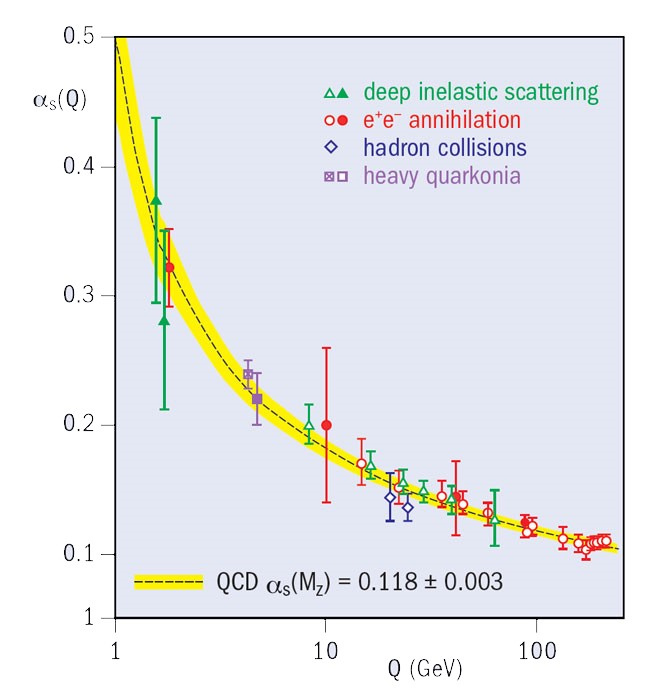
\includegraphics[width=.5\linewidth]{alpha_s.jpg}
\caption{Die Kopplungskonstante der starken Wechselwirkung $\alpha_\text{s}$ in Abh\"angigkeit des Impulsübertrags $Q$. Eingezeichnet befinden sich Messpunkte unterschiedlicher Experimente, sowie in gelb eine theoretische Rechnung.
\cite{article:1}}
\label{fig:alpha_2}
\end{figure}
Anders als die Bezeichnung vermuten l\"asst ist die Kopplungskonstante nicht konstant.
Stattdessen h\"angt $\alpha_\text{s}$ vom sogenannten Impulsübertrag $Q$ zwischen zwei Teilchen ab.
Abbildung \ref{fig:alpha_2} zeigt den Verlauf von $\alpha_\text{s}$ in Abh\"ahngigkeit von $Q$.
Der Impulsübertrag $Q$ h\"angt dabei selbst \"uber die De-Broglie-Wellenl\"ange mit dem Abstand $r$ zusammen.
Es gilt $Q = \frac{h}{\lambda}$, wobei $\lambda$ die r\"aumliche Aufl\"osung beschreibt.
F\"ur eine genau Aufl\"osung, also f\"ur  sehr kleine $r$ muss entsprechend $Q$ gro{\ss} sein.
$\alpha_\text{s}$ h\"angt also antiproportional von $r$ ab.
Aufgrund dieser Abh\"angigkeit von $\alpha_\text{s}$ bez\"uglich $Q$ beziehungsweise $r$ nennt man $\alpha_\text{s}$ auch \textit{running $\alpha_\text{s}$}. 
Den Zustand f\"ur sehr kleine $\alpha_\text{s}$ nennt man asymptotische Freiheit, da sich innerhalb dieses Zustands Quarks und Gluonen quasi frei bewegen k\"onnen.
Um so einen Zustand erzeugen zu k\"onnen braucht man eine hohe Dichte von Quarks und Gluonen oder eine hohe Temperatur.
Eine verbreitete theoretische Beschreibung eines Mediums in diesem hei{\ss}en und dichten Zustand ist das sogenannte Quark-Gluon-Plasma, kurz QGP.
\newline
Ein solcher hei{\ss}er und dichter Zustand entsteht kurz nach der Kollision von zwei hochenergetischen Atomkernen.
Quarks und Gluonen, die aus diesem Medium kommen, m\"ussen, w\"ahrend der sogenannten Hadronisierung, wieder zu Hadronen werden.
Diese Hadronen k\"onnen zerfallen, insofern sie keine stabilen Teilchen sind.
Es kann auch zu ganzen Zerfallsketten kommen, bis die Endteilchen nicht mehr zerfallen.
Je nach dem, wie schnell Teilchen zerfallen, k\"onnen entweder diese oder ihre Zerfallsprodukte gemessen werden und liefern indirekt Aufschluss auf Eigenschaften des hei{\ss}en und dichten Mediums.
\subsection{Messung neutraler Pionen zur Untersuchung des Quark-Gluon-Plasma} \label{s1s3}
Neben der direkten Referenz können in der Untersuchung von pp-Kollisionen auch Informationen über die stark wechselwirkende Materie beziehungsweise über die starke Wechselwirkung selbst gewonnen werden.
pp-Kollisionen haben hierbei den Vorteil, dass sie besser theoretisch verstanden sind als Kern-Kern-Kollisionen.
Dabei führt man unter anderem die  Partonendichtefunktion der Protonen ein, die angibt, wie wahrscheinlich es ist, ein (Anti-)Quark oder Gluon mit einem bestimmten Impulsanteil des Protons vorzufinden.
Dies wiederum ermöglicht genauere theoretische Beschreibungen von pp-Kollisionen, bei denen im engeren Sinne die Partonen, also die (Anti"-)""Quarks und beziehungsweise oder Gluonen, miteinander stoßen.
\newline
Bei einem solchen Stoß entstehen viele neue Teilchen.
Die Produktionsrate der neuen Teilchen wird dabei in einem Spektrum in Abhängigkeit vom Transversalimpuls angegeben.
Der Transversalimpuls gibt dabei den Impulsanteil an, der senkrecht zur Strahlachse eines Kollisionsexperiments liegt.
Der Transversalimpuls wird deshalb betrachtet, da die kollidierenden Teilchen bei einem solchen Experiment keinen Transversalimpuls besitzen und der gesamte Transversalimpuls der entstandenen Teilchen deshalb aus den physikalischen Prozessen während und nach der Kollision kommt.
\newline
Ein mögliches Teilchen, das in Kollisionen produziert werden kann, ist das neutrale Pion.
Dieses wird in dieser Arbeit analysiert und das Spektrum des transversalen Impulses des neutralen Pions in pp-Kollisionen extrahiert.

\section{Experimenteller Aufbau} \label{s2}
\subsection{ALICE} \label{s2s1}
\subsection{elektromagnetische Kaloriemeter EMCal} \label{s2s2}

\section{Analyse} \label{s3}

\subsection{Datenauswahl} \label{s3s1}

\subsubsection{Datensatz} \label{s3s1s1}

\subsubsection{Clusterauswahlkriterien} \label{s3s1s2}

\subsection{Rekonstruktion neutraler Pionen} \label{s3s2}
%Die gewählten \textit{Cluster} nach den Kriterien aus Abschnitt \ref{s3s1s2} bestehen fast ausschließlich aus Photonen, und  Elektronen beziehungsweise Positronen aus der Konversion eines Photons.
\begin{figure}[t!]
\centering
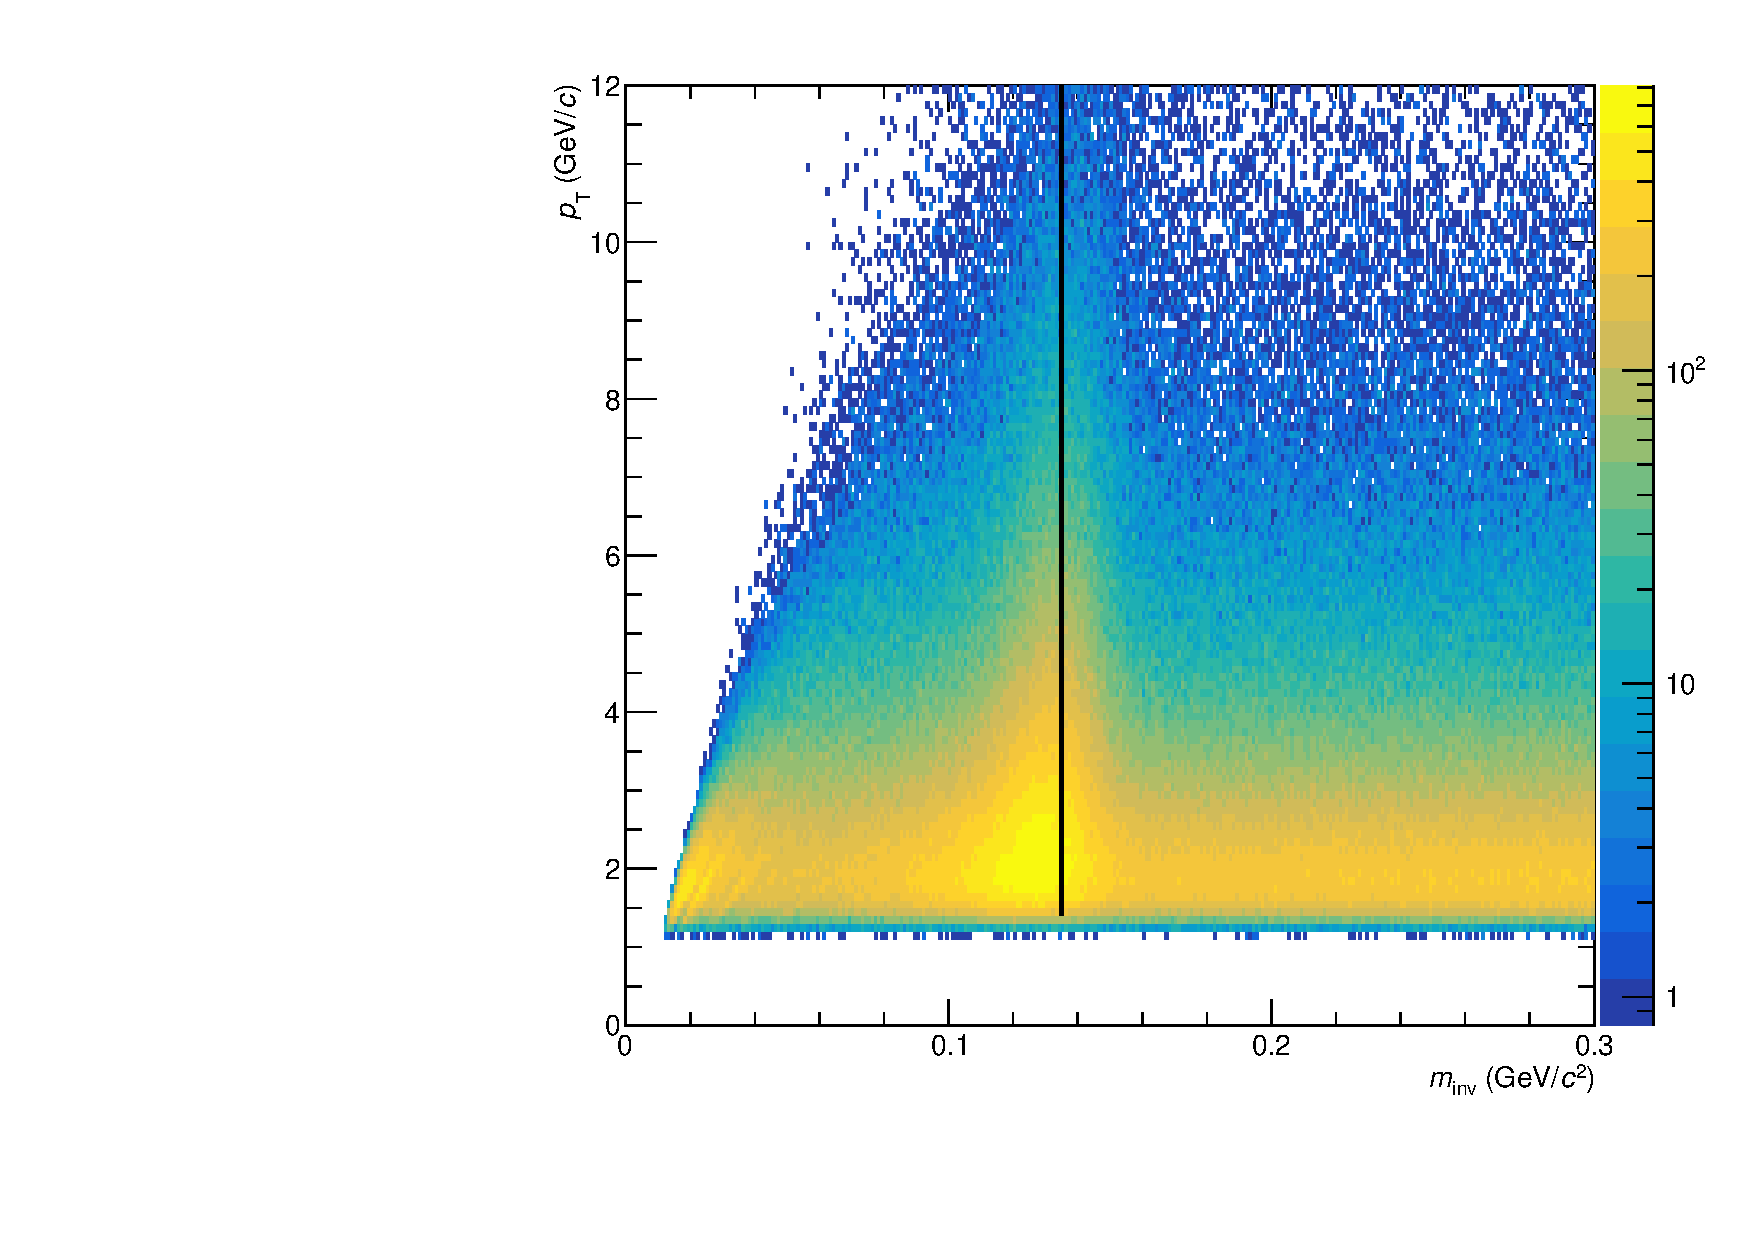
\includegraphics[width=.7\linewidth]{hInvMass_pT_Signal.pdf}
\caption{$p_\text{T}$ und $m_\text{inv}$ als Funktion der Anzahl von kombinierten  Cluster-Paaren aus der gleichen Kollision.
Die rote Linie liegt bei $m_{\text{inv}}\approx0\,135\text{ GeV/}c^{2}$, was in etwa der $\pi^{0}$ Masse entspricht, wo eine deutliche Häufung der Einträge sich abzeichnet.
Die schwarzen Linien stellen die Grenzen der $p_{\text{T}}$-Intervalle dar.}
\label{figInvMassPt_a}
\end{figure}
\newline
Um die Anzahl der detektierten $\pi^{0}$ zu messen, werden von \textit{Clusterpaaren} die invariante Masse und der Transversalimpuls nach Gleichungen \ref{eq_invmass} und \ref{eq_pt} bestimmt.
Da die Information fehlt, ob und welche \textit{Cluster} von einem Teilchen aus dem Zerfall eines $\pi^{0}$ stammen, werden alle \textit{Cluster} eines \textit{events} paarweise mit einander kombiniert.
Diese Methode wird als \textit{same event} Methode bezeichnet.
Abbildung \ref{figInvMassPt_a} zeigt die Anzahl der \textit{Clusterpaare} in Abhängigkeit der invarianten Masse $m_{\text{inv}}$ und des Transversalimpulses $p_{\text{T}}$.
Durch die paarweise Kombination aller \textit{Cluster} eines \textit{Events} gibt es sowohl Kombinationen von \textit{Cluster} von Teilchen die aus dem Zerfall eines $\pi^{0}$ stammen, als auch \textit{Cluster} von Teilchen die nicht über den Zerfall eines einzelnen $\pi^{0}$ zusammenhängen.
\newline
Die Summe aller \textit{Clusterpaare}, die aus einem Zerfall eines $\pi^{0}$ kommen, wird als Signal bezeichnet.
Es zeichnet sich eine Häufung der Datenpunkte um $m_{\text{inv}}\approx 0\,135\text{ GeV}/c^{2}$, also um die Masse des $\pi^{0}$, ab.
Dieser Häufung liegt vor allem das Signal zugrunde.
Da Photonen durch Paarbildung in ein Elektron und ein Positron konvertieren können, bestehen einige\textit{Cluster} aus nur einem der beiden Konversionsprodukte.
Diese \textit{Cluster} besitzen eine geringere Energie, als das eigentliche Photon besaß.
Durch Kombinationen dieser \textit{Cluster} entstehen Einträge bei einer invarianten Masse, die meistens geringer ist als die Masse von $\pi^{0}$, wenn beide Teilchen, die dem \textit{Cluster} zugrunde liegen, dem selben $\pi^{0}$ entstammen.
Deshalb wird bei invarianten Massen $m_\text{inv}<0\,135\text{ GeV}/c^{2}$ ein Teil des Signals erwartet.
\newline
Alle \textit{Clusterpaare}, die nicht zum Signal zählen, bilden den Untergrund, der in zwei Teile unterteilt wird, dem kombinatorischen oder auch unkorrelierten Untergrund und dem korrelierten Untergrund.
Dem korrelierten Untergrund liegen paarweise Kombinationen von \textit{Cluster} zugrunde, zwischen denen eine Korrelation besteht.
Das heißt, dass die Teilchen der zugehörigen \textit{Cluster}, nicht aus dem Zerfall eines einzelnen $\pi^{0}$ stammen, aber über andere Zerfälle zusammenhängen.
Durch die paarweise Kombination von \textit{Cluster} von unkorrelierter Teilchen entsteht der unkorrelierte Untergrund.
\newline
Aufgrund der Anforderung an den Öffnungswinkel werden stetig mehr Kombinationsmöglichkeiten der \textit{Cluster} ausgeschlossen, da ein immer  größerer Anteil der \textit{Cluster} aus zwei Teilchen besteht.
Die ausgeschlossenen Kombinationen liegen im Bereich kleiner invarianter Massen weshalb es bei bei kleinem $m_{\text{inv}}$ keine Datenpunkte gibt.
Das führt dazu, dass mit steigendem $p_{\text{T}}$ immer mehr Signal nicht rekonstruierbar wird.
\newline
Die Anzahl der $\pi^{0}$ weist eine $p_{\text{T}}$-Abhängigkeit auf.
Deshalb wird die Verteilung aus Abbildung \ref{figInvMassPt_a} in einzelnen $p_{\text{T}}$-Intervallen analysiert.
Die Intervalle werden so gewählt, dass sie möglichst klein sind, während die statistischen Unsicherheiten der Datenpunkte nicht zu groß werden.
\begin{figure}[tbp]
\centering
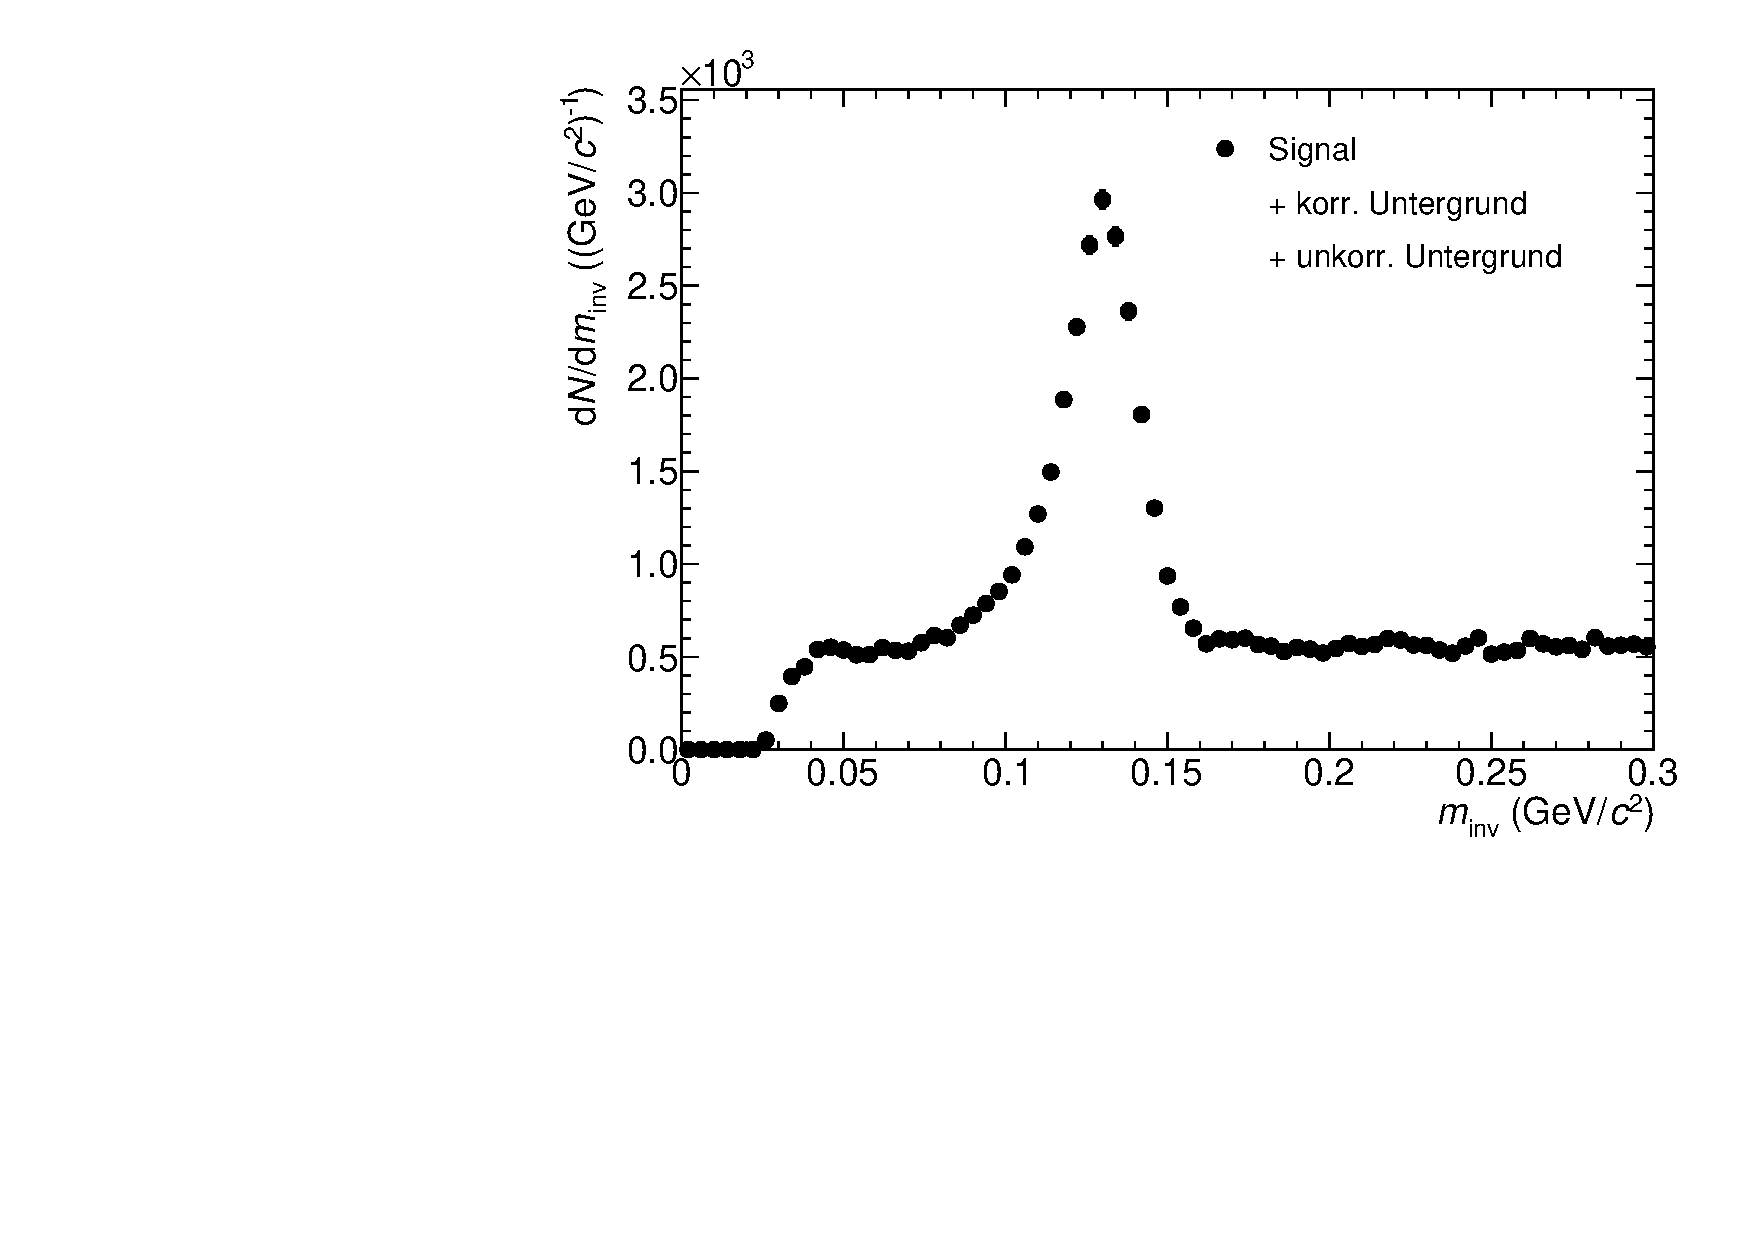
\includegraphics[width=.75\linewidth]{hSignalPlusBkg.pdf}
\caption{Projektion von Abbildung \ref{figInvMassPt_a} im $p_{\text{T}}$-Intervall $(3,2 - 3,4) (\text{GeV/}c)$. Es ist ein deutlicher Peak um $m_{\pi^{0}} \approx 0\,135\text{ GeV/}c^{2}$ zu erkennen, aber auch Untergrund, da das Signal zu höheren Massen gaußförmig abklingen sollte. Bei $m_{\text{inv}} < m_{\pi^{0}}$ kann Signal vorliegen, das aus konvertierten Photonen besteht, weshalb eine Aussage über die Form, beziehungsweise den Untergrund dort schwer möglich ist.}
\label{figSignalPlusBkg}
\end{figure}
\newline
Abbildung \ref{figSignalPlusBkg} zeigt die Anzahl der \textit{Clusterpaare} in Abhängigkeit der invariante Massen im $p_{\text{T}}$-Intervall von $(3\,2 - 3\,4)(\text{GeV}/c)$.
Die in Abbildung \ref{figInvMassPt_a} beschriebene Anhäufung der Datenpunkten zeigt sich auch hier deutlich und wird im Folgenden als Peak bezeichnet.
Der Peak besteht wie zuvor erwähnt hauptsächlich aus Signal.
\newline
Im folgenden Abschnitt wird eine Methode zur Abschätzung des unkorrelierten Untergrunds vorgestellt. 

\subsection{Absch{\"a}tzung des unkorrelierten Untergrunds} \label{s3s3}
%\begin{figure}[tp]
\centering
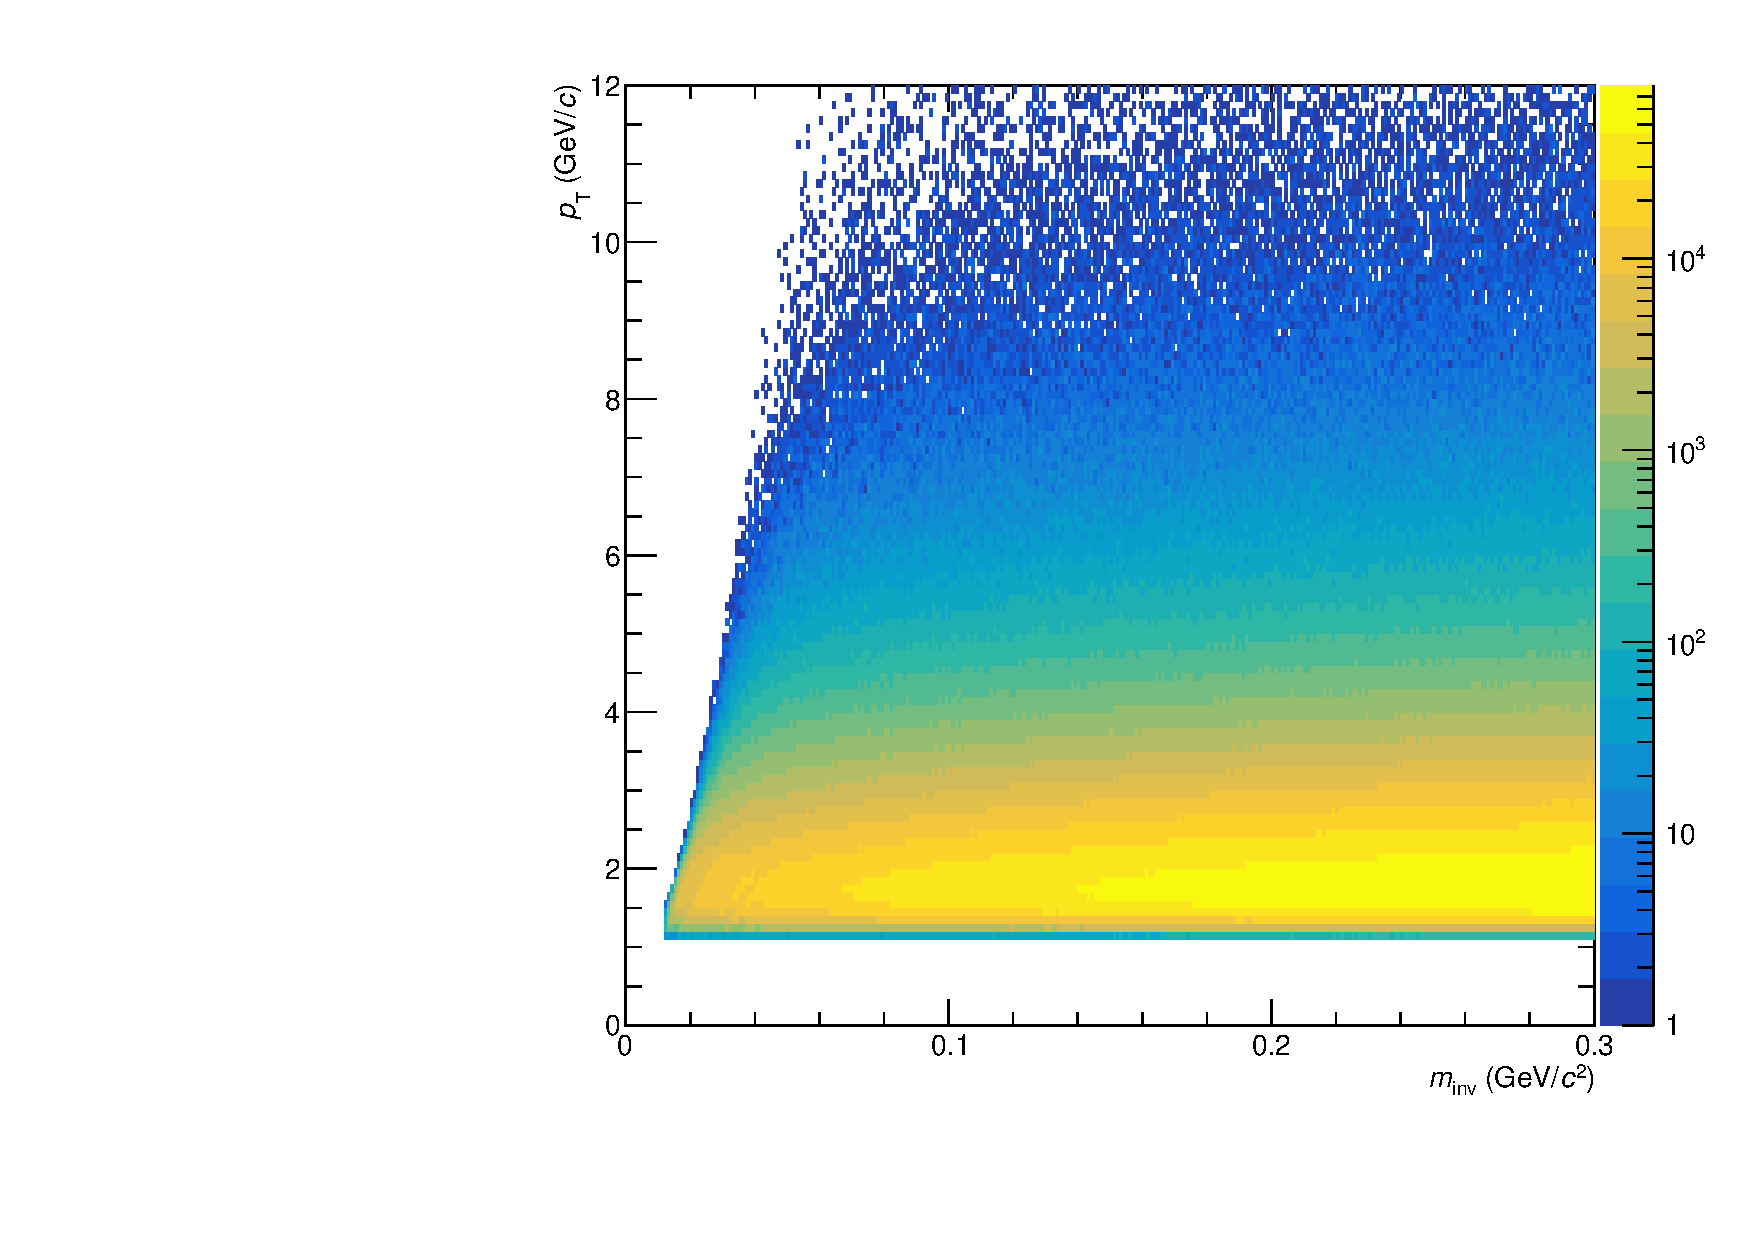
\includegraphics[width=.7\linewidth]{hInvMass_pT_Bkg.pdf}
\caption{$p_\text{T}$ und $m_\text{inv}$ als Funktion von der Anzahl von kombinierten  \textit{Clusterpaaren} aus unterschiedlichen \textit{events}.}
\label{figInvMassPt_b}
\end{figure}
Durch das paarweise Kombinieren aller Photonenkandidaten, wie es in Abschnitt \ref{s3s2} vorgestellt wurde, besteht ein großer Anteil der rekonstruierten Datenpunkte aus unkorreliert Paaren.
Um den unkorrelierten Untergrund abzuschätzen werden Photonenkandidaten aus unterschiedlichen \textit{events} paarweise miteinander kombiniert.
Diese Methode wird als \textit{mixed event} Methode bezeichnet.
Abbildung \ref{figInvMassPt_b} zeigt eine Verteilung, bei der Photonenkandidaten aus unterschiedlichen \textit{events} miteinander kombiniert wurden.
Eine Häufung der Datenpunkte um eine bestimmte invariante Masse gibt es, wie zu erwarten, nicht.
Durch die Anforderungen an den Öffnungswinkel sind wieder keine Datenpunkte bei kleinen invarianten Massen zu finden.
Die untere Grenze, ab welcher invarianten Masse Kombinationen möglich sind steigt mit $p_\text{T}$, analog wie zuvor bei Abbildung  \ref{figInvMassPt_a}.
\newline
In der \textit{mixed event} Methode gibt es eine größere Anzahl an Kombinationsmöglichkeiten, als in der \textit{same event} Methode.
Daraus resultiert eine größere Anzahl an Einträgen in der Verteilung der invarianten Masse und des Transversalimpulses, weshalb die Verteilung, die aus der \textit{mixed event} Methode kommt, skaliert werden muss an die Verteilung aus der \textit{same event} Methode.
Die Skalierung erfolgt bei $m_\text{inv} \in \left[0\,19,3\,0\right] (\text{GeV/}c^{2})$, da dort kein Signal erwartet wird.
Es ergibt sich für den Skalierungsfaktor:
\begin{align}
\label{eqBackSkalierung}
\alpha &= \frac{\sum_{i \neq j}\sum_{n}m_{\text{inv}}\left( \gamma^{(n)}_{i},\gamma^{(n)}_{j}\right) }{\sum_{i,j}\sum_{n \neq m}m_{\text{inv}}\left( \gamma^{(n)}_{i},\gamma^{(m)}_{j}\right) }
\end{align}
Die oberen Indize $m$ und $n$ stehen hierbei für ein Event, aus dem ein Photon kommt und die unteren Indize $i$ und $j$ numerieren die Photonen ($\gamma$).
\begin{figure}[tp]
\centering
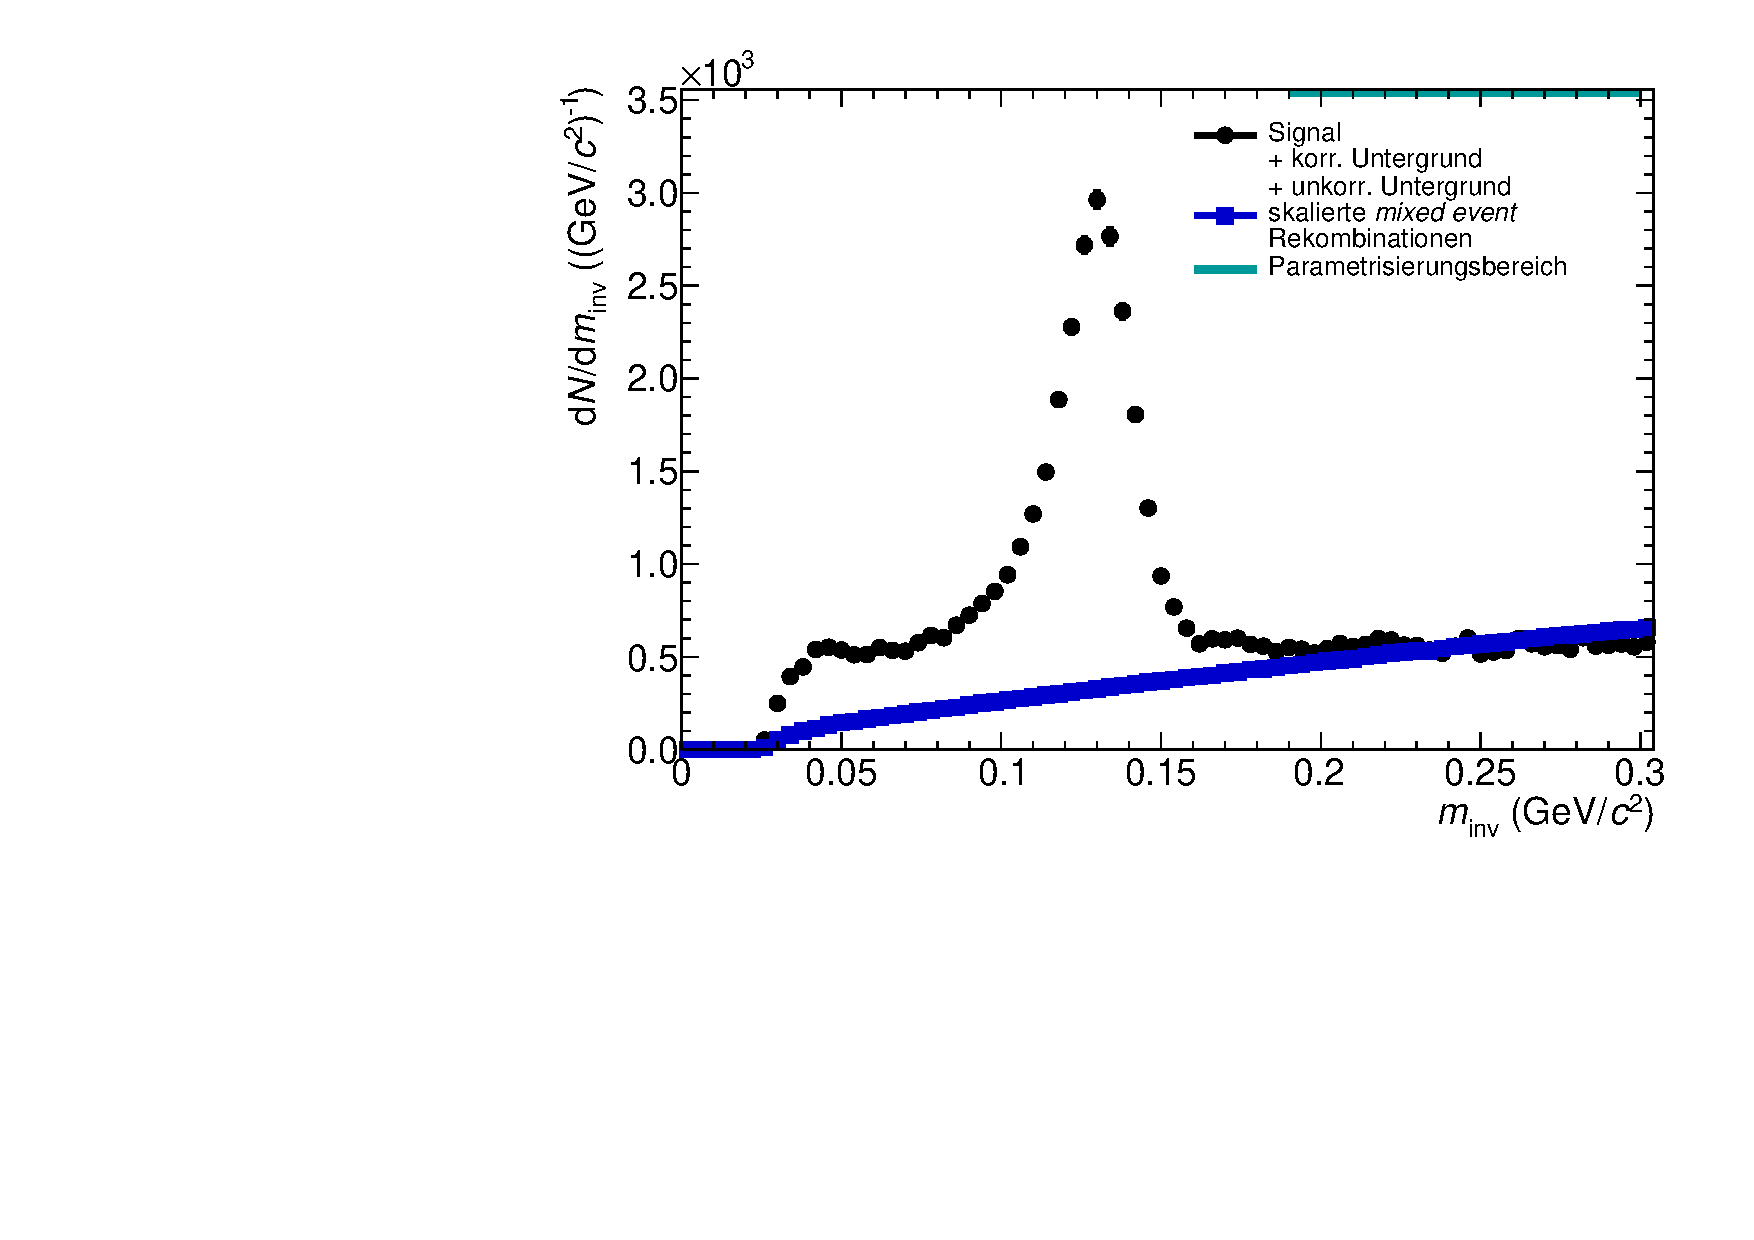
\includegraphics[width=.75\linewidth]{hUncorrBkgNorm.pdf}
\caption{Nach Gleichung \ref{eqBackSkalierung} skalierte {\it mixed event} Kombinationen als Abschätzung des unkorrelierten Untergrunds zusammen aufgetragen mit Signal zuzüglich beiden Untergrundkomponenten wie in Abbildung \ref{figSignalPlusBkg}.}
\label{figUncorrBkgNorm}
\end{figure}
\newline
Abbildung \ref{figUncorrBkgNorm} zeigt die skalierten \textit{mixed event} Kombinationen und das Signal zusammen mit dem korrelierten und dem unkorrelierten Untergrund.
Nachdem der unkorrelierte Untergrund abgeschätzt wird, wird dieser von der Verteilung der invarianten Masse aus der \textit{same event} Methode subtrahiert.
\begin{figure}[tp]
\centering
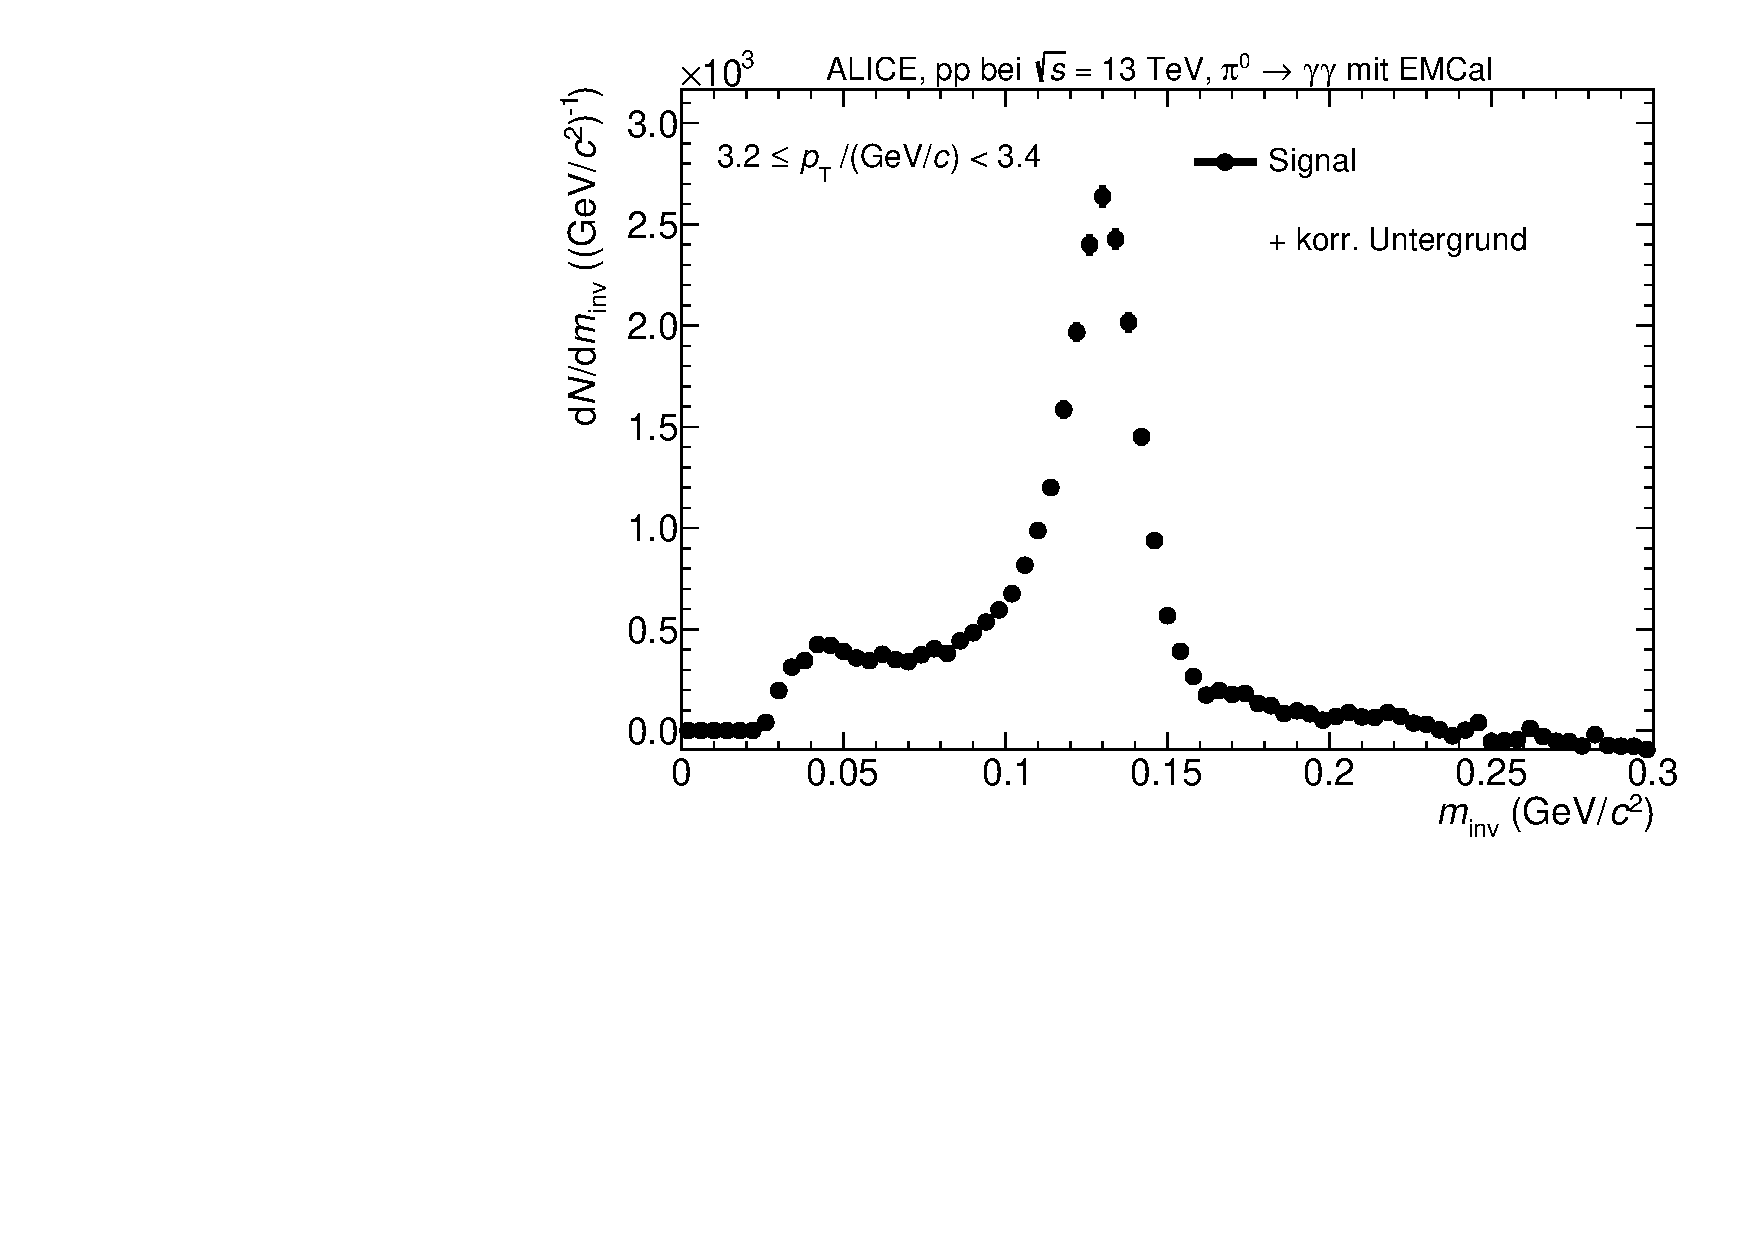
\includegraphics[width=.75\linewidth]{hInvMass_Data.pdf}
\caption{Signal nach Abzug des unkorrelierten Untergrunds.}
\label{figInvMass_Data}
\end{figure}
\newline
Abbildung \ref{figInvMass_Data} zeigt eine Verteilung der invarianten Masse aus der \textit{same event} Methode, nachdem die skalierten Kombinationen aus der \textit{mixed event} Methode, als Abschätzung der unkorrelierten Untergrunds, abgezogen wurden.
%Da Photonen durch Paarbildung in ein Elektron und ein Positron konvertieren können, bestehen einige Photonenkandidaten aus \textit{Clustern} aus nur einem der beiden Konversionsprodukte.
%Diese Photonenkandidaten weisen dann eine geringere Energie auf, als das eigentliche Photon besaß.
%Durch Kombinationen mit diesen Photonenkandidaten entstehen Einträge bei einer invarianten Masse, die meistens geringer ist als die Masse von $\pi^{0}$, obwohl beide Photonenkandidaten dem selben $\pi^{0}$ entstammen.
%Deshalb wird bei kleineren invarianten Massen links vom Peak ein Teil des Signals erwartet, jedoch auch korrelierter Untergrund.
\newline
Der nächste Schritt in der Analyse neutraler Pionen ist die Bestimmung des korrelierten Untergrunds.
Das Abschätzen mit einer linearen Funktion hat sich als gängigste Methode zur Abschätzung des korrelierten Untergrunds entwickelt und wird im Folgenden als Standardmethode bezeichnet.
In dieser Arbeit wird der korrelierte Untergrund sowie das reine $\pi^{0}$-Signal mit Hilfe von Monte Carlo Templates bestimmt.
Die Ergebnisse der Analyse mit Hilfe von Monte Carlo Templates, sowie mit der Standardmethode werden miteinander vergleichen, um eine Aussage über den möglichen Nutzen von Analysen mit Hilfe von Monte Carlo Templates treffen zu können.
Im folgenden Abschnitt wird zunächst die Standardmethode kurz erläutert.
\subsection{Peak Extraktion mit Hilfe von Parametrisierungen von Funktionen} \label{s3s4}

\subsubsection{Absch{\"a}tzung des korrelierten Untergrunds} \label{s3s4s1}

\subsection{Peak Extraktion mit Hilfe von Parametrisierungen von Templates} \label{s3s5}

\subsubsection{Template des Signals} \label{s3s5s1}

\subsubsection{Template des korrelierten Untergrunds} \label{s3s5s2}

\subsubsection{Parametriesierungsmethode} \label{s3s5s3}

\subsubsection{Abzug des korrelierten Untergrunds und Integration des Signals} \label{s3s5s4}

\section{Korrigierter Yield} \label{s4}

\subsection{Korrekturen} \label{s4s1}

\subsection{Systematische Unsicherheit} \label{s4s2}

\section{Zusammenfassung und Ausblick} \label{s5}


\end{document}
